\documentclass{article}

%TODO WHY ?
\usepackage{standalone}

%TODO WHY ?
\usepackage[utf8]{inputenc}

\usepackage{geometry}
\usepackage{graphicx}
\geometry{hmargin=2cm,vmargin=1.5cm}


%TODO WHY ?
\usepackage[utf8]{inputenc}
\usepackage{relsize}

%TODO WHY ?
\usepackage{amsmath,amsfonts,amssymb}

\setlength\fboxrule{3pt}

%TODO WHY ?
\usepackage{gensymb}

%TODO WHY ?
\usepackage{import}


%disable indentations
\setlength{\parindent}{0pt}

%Color definition TODO CHECK
\usepackage{xcolor}

%Code listings
\usepackage{listings}

\definecolor{mGreen}{rgb}{0,0.6,0}
\definecolor{mGray}{rgb}{0.5,0.5,0.5}
\definecolor{mPurple}{rgb}{0.58,0,0.82}
\definecolor{backgroundColour}{rgb}{0.95,0.95,0.92}

\lstdefinestyle{CStyle}{
    backgroundcolor=\color{backgroundColour},   
    commentstyle=\color{mGreen},
    keywordstyle=\color{magenta},
    numberstyle=\tiny\color{mGray},
    stringstyle=\color{mPurple},
    basicstyle=\footnotesize,
    breakatwhitespace=false,         
    breaklines=true,                 
    captionpos=b,                    
    keepspaces=true,                 
    numbers=left,                    
    numbersep=5pt,                  
    showspaces=false,                
    showstringspaces=false,
    showtabs=false,                  
    tabsize=2,
    language=C
}





\begin{document}

    \tableofcontents

%    \section{Solving models}

\subsection{Primary considerations}

Suppose that we want to control a robot.
We will take two examples of the stepper controlled CNC and a quadrirotor, both apparently having different control models.\newline

Due to its stepper motors, and the supposition that no forces will interfere, the CNC can be controlled in a deterministic way, with no feedback.
The drone, is submitted to the gravity and therefore, is controlled using feedback algorithms, to adjust motors powers in real time.\newline

Beyond those differences, those robots have similarities
\begin{itemize}
    \item [.] They are represented by a state.
    For the CNC, it can be the set of coordinates of its steppers, their speed, acceleration, etc\ldots
    For the drone, it can be, is the set of powers of its motors, and angular positions, speeds, accelerations\ldots
    \item[.] They are solved, ie, an algorithm is used to determine, knowing the current state, the target state.
    For the CNC, it can be a trajectory tracer, for the drone, it can be a set of PIDs, coupled with a trajectory tracer;
    \item[.] They are controllable, ie, the solving algorithm takes parameters that determine its behaviour.
    For the CNC, it can be the acceleration / speed bounds of stepper motors, the number of steps per unit, etc\ldots
    For the drone, it can be PID coefficients.\newline
\end{itemize}

We hereby see that behind those control problems, there are common elements.\newline

An approach, when writing a control algorithm for one of these, can be to neglect those similarities, and build a specific control algorithm.
Another approach that motivates this section, is to evaluate this range of problems in a more abstract way.\newline

The idea here is not to search for similarities in solutions to those problems, but rather to start from an abstract
model of solving system, of which those control problems are particular cases.

%TODO FINISH THE INTRODUCTION, WHY ARE WE BUILDING THIS MATHEMATICA ABSTRACT ?


\subsection{Solving system}

Let $S, C$ be sets, $X : S \times C \rightarrow S$, the triplet $(S, C, X)$ is a solving system;

S is the system's states set.
C is the system's control set.
X is the system's solver.

$S \in S$ is a state.\newline
$c \in C$ is a control element;

A state $s \in S$ can be seen as one representation of a particular system, S being the set of all possible states.
A state can be known, or not, and the aim of a solver will be to compute it.\newline
A control element $c \in C$ can be seen as a set of parameters that will affect the computation of a state, during a solving process.
All of these parameters are know, they do not intend to be determined by the solver, but to control is behaviour


A state $s$ can represent a robot's physical state, (see behind), or the various variables of an equation system,
generally, any set of variable that must be computed;
A control element $c$ can contain acceleration bounds for the trajectory controller of the robot,
or coefficients of the equation system.


\subsection{Solving system}



%    \newpage

\section{Introduction}


\subsection{Primary goals and definitions}

Let a machine, whose behaviour we wish to control;\newline

The machine is defined by a set of $n$ actuators, a control system of size $n$, a geometric model, and a kinematic
model;\newline

The control system is coordinate system that is easier to manipulate, or that has more physical meaning than the
actuator's system.\\
For example, a 6DOF arm's actuator system has no direct spatial meaning, and spacial trajectory are very difficult
to express in it.\\
Target positions and speeds will be expressed in this system;\newline

The geometric_model is the function that will be used to convert control positions to actuators positions;


\subsection{Notations}

Throughout the rest of this document, we will use the following notations :\newline

$E = {i\in \{0, n-1\}}$.\newline

$i$ is the index of an actuator or of an axis of the control system, $E$.\newline

$A_i$ is an actuator.
\begin{itemize}
    \item[-] $u_{i_A}$ is its unit;
    \item[-] $D_{i_A}$, an interval included in $\mathbb{R}$ is its domain;
    \item[-] $p_{i_A}$ is its position expressed in $u_{i_A}$;
    \item[-] $v_{i_A}$ is its speed, expressed in $u_{i_A} \cdot s^{-1}$
    \item[-] $a_{i_A}$ is its acceleration, expressed in $u_{i_A} \cdot s^{-2}$\newline
\end{itemize}

$C_i$ is an axis of the control system.
\begin{itemize}
    \item[-] $u_{i_C}$ is its position;
    \item[-] $D_{i_C}$, an interval included in $\mathbb{R}$ is its domain;
    \item[-] $p_{i_C}$ is its position expressed in $u_{i_C}$;
    \item[-] $v_{i_C}$ is its speed, expressed in $u_{i_C} \cdot s^{-1}$
    \item[-] $a_{i_C}$ is its acceleration, expressed in $u_{i_C} \cdot s^{-2}$\newline
\end{itemize}

$g :  \prod\limits_{i\in E} D_{i_C} \rightarrow \prod\limits_{i\in E} D_{i_A} $,
$ (p_{i_C})_{i \in E}\rightarrow (p_{i_A})_{i \in E}$\newline

is the geometric_model function, that translates control positions into actuators positions;


\newpage

\subsection{Machine state}

The state of the machine at a given time is defined by the following set of variables

\begin{itemize}
    \item[-] $u_{i_C}$ its control positions;
    \item[-] $v_{i_C}$ its control speeds;
    \item[-] $u_{i_C}$ its actuation positions;
    \item[-] $v_{i_C}$ its actuation speeds;
\end{itemize}

There is a direct relation between control and actuation positions, and control and actuation speeds, given by
the geometric_model function, but not between actuation positions and speeds, or control positions and speeds;\newline

To change the state of the machine, we execute a movement.\newline

A movement is defined by :
\begin{itemize}
    \item[-] $d_i$ its actuation distances. Distances could also be expressed in the control system,
    but it makes more sense to consider them in the actuation system, as actuators do the final
    movement;
    \item[-] $t$ its duration;
\end{itemize}


\subsection{Physical limitations}

The machine is controlled by actuators, that can be positioned at any point of their domain, without restrictions.
\newline

However, precautions must be taken when attempting to move them. Each type of actuator has its own kind of speed
limitations, often correlated with the geometric_model;\newline

For a given actuator, part of a machine, variation of the speed must be carefully monitored.
If speed constraints are not met, actuators may halt, or be damaged, which in both case, would compromise the
machine's integrity;\newline


%    \newpage

\section{Control Model}


\subsection{Position target : what we want to do}

Controlling the behaviour of the machine, in the less restrictive meaning, means determining successive actuation
distances, and time intervals between them.\newline

Ideally, we would like to determine consecutive positions (in any of the two coordinate systems), then determine
actuation distances, and determine time intervals so that speed of a group of axis (in any of the two coordinate
systems) matches a target one;\newline


\subsection{Physical limitations : what we can do}


However, this is not so simple. Indeed, the fact of determining target distances for each actuator, at a given
state, will by itself impose constraints on the time;\newline

Suppose the machine in the state S. We wish to execute a movement, whose actuation distances have been computed.\newline

Actuators are at a determined speed, and still have physical limitations. It is important to mention here that
actuators are all moved simultaneously.\
    Therefore, the time we choose for this movement will determine actuators speeds. But as we said previously,
the variation of actuators speeds can't be set randomly without risking to damage actuators and the machine;\newline

More formally, given a machine state S and a set of actuation distances $(d_i)_i$, each actuator will provide a
duration interval $I_i = [t_{i_{\min}}, t_{i_{\max}}]$ that is acceptable for it;\newline

Given this set of intervals, we must choose a duration $t$ that respects all time constraints, ie
$d \in \bigcap \limits _{i \in E} I_i$\newline

What now if $\bigcap \limits _{i \in E} I_i = \emptyset$ ?\newline

This means that the movement we are trying to execute is simply non realisable. This is caused by two time
intervals that do not intersect, ie two actuators, that have incompatible speed variations : there is no compatible
duration for one to decelerate slowly enough, and for the other to accelerate slowly enough;
\footnote{This sentence can lead to assume erroneously that speed limitations only reside in their derivative,
which might be true in simple machines, but in more complex ones (robotic arms for ex), may not be always the
case.}\newline

There are two potential solutions to this problem.\newline

The naive (but simple !) solution, is to select an arbitrary time, given an absolute criteria. We could for example
select a time that would limit acceleration, but break deceleration rules. The two great advantages of this
solution are to respect required movement distances, and to require few calculation; The disavantage is that it
breaks actuations limitations\newline

The second solution complements the first one by modifying movement distances to match actuators limitations.
Now that we have determined our movement time, we will modify movement distance for actuators that see their
limitations broken; This solution makes the assumption that the movement distance that matched speed limitations
for a given time can actually be determined.\
    If so, this method will give a movement that can be safely executed by all actuators in its duration.\newline

For now, we have determined movement distances, and a time interval in which we can safely choose the movement
duration. This interval can be of length 0, and then we have no choice on the duration;\newline


\newpage

\subsection{Kinematic constraints : what we choose to do}

Now that we have a determined set of movement distances, and a variable duration, we can select the most relevant
duration.\newline

We could, for example, restrict again the duration interval, to values that match acceleration bounds on a control
axis.
It could also be possible to verify that a deceleration is required to satisfy eventual jerk bounds on a control
axis.\newline

More generally, the selection of the duration comes by consecutive restrictions of the duration interval by ordered
optional constraints;
These constraints are functions that take the current state of the machine and provide a duration bound.
They are qualified optionnal because the final duration will necessarily be in the interval that satisfies actuators
constraints;
They are qualified ordered because a constraint will evaluated only if the interval is not of length 0;\newline

There can be as many constraints as we want. They are evaluated in order until interval is of length 0, or until
all have been evaluated;
If all constraints have been evaluated and the duration interval is not of length 0, the upper duration is selected;
\newline



    
\newpage

\section{Planner}

This section describes the planner algorithm implemented in the project.
\newline

Suppose we have access to a system whose behaviour must be controlled. 
This system must follow a sequence of trajectories, trajectories that define a sequence of target positions
the system will have to reach.
As it is possible for the system to reach these positions, it is also possible that it does not. 
Some external perturbations may affect the system, that would not reach its target positions.
Considering those perturbations forces to generate a target position knowing the system's current position.
The system will be said to be controlled in closed loop.

Theoretically, any point of any trajectory is a potential target.
The only pieces of informations we have to decide which point to choose are : 

\begint{itemize}

\item[-] the current position of the system; this information gives a way to compare two candidate target
points. Their positions relatively to the current position will help to decide which one to choose. 

\item[-] the previous target point, or the start position; this information gives a position to start 
searching for a target point; 

\end{itemize}

That being said, the generation of a target positon appears \footnote{and obviously is} a complex process.

A particular algorithm, called a planner, will be used for this purpose.

A planner is an algorithm that, given a sequence of trajectories, a point of a trajectory to start searching 
at, and a current position, searches the trajectories sequence from the start point for a valid target
position.

newline

In order to describe its main objectives more accurately, we need to elaborate a bit on the notion of 
trajectory.
\newline

\subsection{Trajectory}

Definition : a trajectory t is a continuous application from a segment of R in $R^n$ :
\newline

$t : [a, b] -> R^n$, $a$ and $b$ two real numbers, $n$ a positive integer, t continuous.
\newline

Naming convention : 
\begin{itemize}
\item [-] n : the dimension of the trajectory;
\item [-] x in [a, b] : an index of the trajectory;
\item [-] t(x), x in [a, b] : a point of the trajectory;
\item [-] a : the minimal index, the initial index;
\item [-] t(a) : the initial point;
\item [-] b : the maximal index, the final index;
\item [-] t(b) : the final point;
\newline
\end{itemize}

A trajectory $t$ represents a path in a particular space from its initial point $t_i$ to its final point 
$t_f$.

Its aim is to fully determine the path that some system must follow in this space;


\subsection{Target point choice}

As we stated earlier, any point of any trajectory is a candidate target, and the planner has to choose 
between all those possible points.
To do this, the planner considers the distance between a candidate target, and the current position.

The planner is given a positive interval, called the target interval, with the objective to
find a point of a trajectory whose distance from the current position belongs to the target interval.

Given the current position, the target interval defines a set of valid points, that verify the distance 
condition. 

The sequence of trajectories may or may not intersect this set in several portions of trajectories.

The planner must at first determine these candidate portions. Several parameters may influence the 
search. Among these parameters, is or is not the start position, that gives a point in the trajectory to start
searching at. 

When the planner has finished searching for candidate portions, it must choose a point in one of them. 
Many parameters may influence the choice. If trajectories must be followed in order, the planner may choose
the closest portion of trajectory to start point, and choose a point close to a distance target. 

If trajectories may be skipped, at the benefit of the traversal speed, the planner may choose the last 
candidate portion (closest to the end of the sequence), and also, choose a point close to a distance target.


\subsection{Hook mode}

No constraint has been imposed on trajectories in the trajectory sequence, except that trajectories must be 
continuous. Successive trajectories may be disjoint, ie, have separate initial and final points.

When reaching the final position of a trajectory, and attempting to reach the initial point of the next
trajectory, if the distance between stated points does not belong to the target interval, no valid target
point may be found.




%TODO REWRITE THIS
Let us consider now, two trajectories, $u$ and $v$ that share the same dimension, and must be followed one 
after the other, $u_i$, $u_f$, $v_i$, $v_f$ initial and final points of $u$ and $v$.
If both trajectories are joint, ie $u_f = v_i$, the path between $u_i$ and $v_f$ is fully determined.
If trajectories are disjoint, the path is simply undetermined, as there is no trajectory defined between
$u_f$ and $ v_i$to do so.
\newline

A planner can accept only a sequence of consecutively joint trajectories, or can accept any sequence of 
trajectories.
In the second case, it must contain a hook algorithm, that is in charge of determining an arbitrary path
from $u_f$ to $ v_i$.
The planer has to work modes, trajectory mode, where it processes a trajectory, and hook mode, where it 
attempts to reach a trajectory's initial point;

\newpage


\subsection{Transition point}

A transition point is a point where a brutal change of direction occurs.
\newline

As a planer can be used to control physical systems, that may suffer of this kind of changes, it may be 
important to monitor the existence of those points.
A planner can offer this monitoring, so that actions can be taken by another piece of code.
\newline

The presence of transition points inside trajectories is uncertain, and must be determined manually;
A planner can also offer this functionality, but it involves traversing the trajectory entirely, and 
it can be heavy for some low-performance systems;
\newline

However if we cannot easily detect transition points inside a trajectory, there are two immediate 
transition points, at extremal indices.
\newline

When completing a trajectory (reaching its final point), the planner may, enter into hook mode.
The hook algorithm is used to determine a path to the next trajectory's initial point.
This is the first transition point, as the direction the planner takes may not be the direction at the end
of the trajectory;
\newline

When the hook algorithm manages to reach the next trajectory's initial point, the planner goes into 
trajectory mode, and starts searching the trajectory for an adequate point.
This is the second transition point, as the direction the next trajectory takes may not be the direction 
the planner took to reach its initial point.
\newline


\subsection{Managing transition points}

The planner maintains a list referencing transition points in their order of appearance in the global 
path;
\newline

This list verifies the following conditions :
\begin{itemize}

\item[-] when the planner has processed all trajectories, the list is empty;

\item[-] when the planner is processing a trajectory, the first transition point in the list corresponds to 
the currenttrajectory's final point;

\item[-] when the planner is hooking the next trajectory, the first transition point in the list corresponds
to the initial point of the trajectory to hook;

\end{itemize}

This list is updated the following way :

\begin{itemize}

\item[-] When adding a trajectory to the planner's list, the planner determines if the trajectory is joint to 
its predecessor.
If so, it modifies the last transition point, to reflect the direction change due to the trajectory, 
and marks the transition to trigger trajectory mode.
If not, it modifies the last transition point, to reflect the direction change due to the hook algorithm, 
and mark it to trigger hook mode;
it then adds a transition point to monitor, at the initial point of the new trajectory, to reflect the 
direction change between the hook aglorithm and the trajectory;
Then, it attempts to find transition points in the trajectory.
If it finds some, it adds them in their order of appearance;
As stated earlier, this operation is time-consuming, and can be skipped.
Finally, it creates another transition point to monitor, representing the stop at the end of the new 
trajectory. This transition will be modified, when a new trajectory will be added, as described just before, 
to reflect a direction change instead of a stop.

\item[-] When processing a trajectory, when a transition point is reached inside the trajectory, the planner 
removes the first transition point of the list;

\item[-] At trajectory mode exit, when the planner reaches the last point of a trajectory, or at hook mode 
exit, when the planner has hooked the first point of a trajectory, it removes the first transition point, 
and depending on its type, it enters into hook mode, or trajectory mode;

\end{itemize}

\newpage

\subsection{Trajectory mode}

Following a trajectory is a primary objective for a control system. It is the base objective.
The planner's objective is to decide of a target position. After this decision, multiple corrections
or error sources, or perturbations may intervein, that the planner will not be aware of. 
This will result in a final position that may not be the one the planner previously picked. 
Because of this, to choose a target point, the planner must take the current known position into account.
\newline 

The planner will comprise an algorithm whose purpose is, given a position $P$ (that may not belong to 
the trajectory),to select a point of the trajectory that verifies a distance condition.
For example, the planner may have to pick a point of the trajectory whose maximal or minimal or average 
distance from the provided position is within a certain range $[d_{min}, d_{max}]$.
\newline

More verbosely, the planner disposes of a distance function $d : R^n \times R^n \rightarrow R^+$, 
that takes two points in arguments, and returns a real number, that we will call the distance.
It also posseses a target interval $I = [d_{min}, d_{max}]$ , and a distance target $d_{target}$, that verify
 $d_{min} < d_{target} < d_{max}$.
The planner's goal will be to find a point $Q$, as $d(P, Q) \in I$, as close as $d_{target}$ as possible.
\newline

Given $t$ a trajectory to process, $P$ the position, $d$ the distance function, we can define $D$ the reduced
 distance function :
$D : R \rightarrow R^+, i -> d(P, t(i))$ 
that gives the distance from the position of the point of $t$ at index i.
This function will indicate the planner if a point is close enough to the current position to be considered
as already visited. 
\newline

The objective of the planner is, given a position $P$, a trajectory $t$, a distance function $d$, 
a probable index $i_e$ (e for estimate), and a probable index delta $\delta _i$ to determine, in a minimal 
number of computations, an index $i_f$ (f for final) as $f(i_v)) \in [d_{min}, d_{max}]$.
$i_e$ and $\delta _i$ are two important parameters. The first will determine the first index whose distance
should be computed. If its distance is not in the target interval, $\delta _i$ will be used, to determine the
next point to be evaluated. 
\newline 

This problem as it is a classical analysis problem, and can be solved with many methods;
Though, an aditional rule comes to complexify the resolution. 
Indeed, as the planner's goal is to traverse the whole trajectory, it should prioritise points with high
indices. A simpler rule that is not equivalent but easier to work with, is that the cost should increase 
when increasing the index, at the choosen point.
\newline

A fact to remember, is that the index where the search begins is purely speculative. In case of inacurate 
prediction, different cases can occur.

\newpage

\subsection{Prediction}

We develop here the first stage of the determination of a point. Depending on the exactitude of $i_e$, several
cases are encountered.

\begin{figure}[!h]
\fbox{\centerline{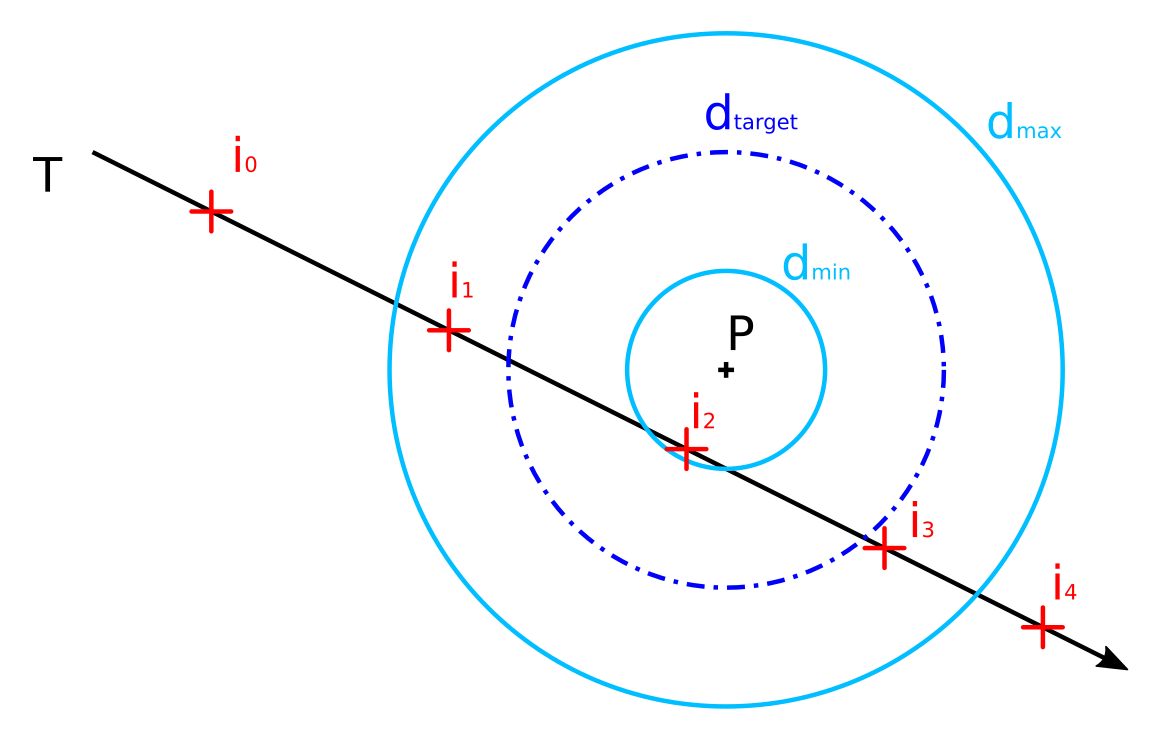
\includegraphics[width=12cm]{sections/traj_cases.png}}}
\caption{Different cases, depending on the index prediction}
\end{figure}

The figure behind shows different cases that may occur, for different values of $i_e$, with a simple example :
the trajectory $T$ to follow is a simple 2D line, and the distance considered is the geometric distance.
$P$ the current position, and circles delimitating the acceptable positions set are drawn accordingly.

Different cases are : 
\begin{itemize}

\item [-] $i_0$, critical traction : $i_e$ is highly underestimated, the distance to the posion being
superior to the maximal bound, incrementing the index making this distance decrease. In this situation, simply
increasing the index until a valid one is found is not enough, because it would lead to choose a point where
the previously enounced rule doesn't apply. In this case, the planner must increase the index, until the 
distance starts increasing and consider points beyond that index only.

\item [-] $i_1$, ghost traction : same case as before, but this time, the estimation gives a valid distance. 
This case is a little bit problematic, as the estimation seems to be valid, but is a matter of fact, 
counterveins to our decision rule. In this case again, the index must be increased until the distance 
increases, and only consider points beyond that index.

\item [-] $_i2$, traction : the prediction lead to a point too close to the current position. This point is 
already visited, and can't be selected. Once again, the index must be increased until the distance increases
, and only indices beyond must be considered during the search.

\item [-] $i_3$, correct prediction : the prediction lead to an acceptable point.

\item [-] $i_4$, resistance : $i_e$ is overestimated, the distance to the position being superior to the
maximal bound, incrementing the index making this distance increase. A suitable point must be seatched before
the estimated index.

\end{itemize}

\newpage

\subsection{Search procedures}

In the list behind, two procedures were implicitely refered : 
\begin{itemize}

\item[-] the slide. Given two indices and their associated distances, the trajectory is traversed in the 
local descending direction, until a local minimum is found, or until the distance decreases 
over a certain target value, or the slide arrives to an extremal index;

\item[-] the raise. Given two points, and their associated distances, the trajectory is traversed in the
local descending direction, until a point at a sufficient distance is found, or the raise reach an extremal 
index;

\item[-] the windowing. Given two points, and their associated distances $d_0$ and $d_1$, 
the trajectory is traversed until a point at a position belonging to an interval 
$D \in [d_0, d_1]$ is found.

\end{itemize}


\subsection{Algorithm}












At the beginning stage of the algorithm, only the point at $i_e$ and its distance are computed.
No indication is available on how the distance will vary when the index does. 
As you may have seen, this information alone does not suffice to determine in which case 
we are.
We can only determine that we are in $i_1$ or $i_3$, or that we are in $i_2$, or that we are 
in $i_0$ or $i_4$.
To go further, a second point will be determined, its index being given by $\delta _i$, and different actions
will be taken.
\newline

Different cases are : 

\begin{itemize}

\item[-] $i_1$ or $i_3$ : within the acceptable bounds : 
the second point is used to determine the current case.
If the distance increases when the index increases (positive derivative), we are in case 
$i_3$ and the point is acceptable. 
If not, we are in case $i_1$, and a slide must be executed.
At the local minimal point, we are either in case $i_3$, which gives us an acceptable point, or in case $i_2$.

\item[-] $i_2$ : below the minimal distance : the estimated point is considered as already visited. 
A raise must be executed, to the minimal distance.
If a point below the maximal distance is found, we are in $i_3$, which gives us an acceptable point.
If a point beyond the maximal distance is found, the windowing gives us an acceptable point.
If no point is found, the trajectory is finished.

\item[-] $i_0$ or $i_4$ : beyond the maximal distance :
the second point is used to determine the current case.  
If the distances increases with the index increasing, we can suppose we are in $i_4$. If not, we are in $i_1$.
A slide is executed, targetting the maximal value, if we are in $i_1$. If in $i_4$, we need to 
reach the minimum.
Here comes a problem : there is no guarantee that the local minimum is in the distance bounds, as the
direction to take is extrapolated from evaluated points, which has no guarantee to be accurate. 
There is either no guarantee that a point in the distance bounds exists, as the current position could be too
far from the trajetory.
If we are in $i_4$, if a local minimum was detected, and the maximal distance has never been reached, 
the planner has failed to compute the point. If the maximal distance has been reached, we either 
have determined a valid point, or can use the windowing to compute one.
If we are in $i_1$, and the local minimum is not lower than the maxmal distance, the planner has failed to 
compute the point. If not, we end up in $i_3$, which gives us a valid point, or in $i_2$, which leads us to 
a valid point.

\end{itemize}

\newpage

\subsection{Limit cases}




\subsection{Faults}

\subsection{Interrupt levels}



    \newpage

\section{Planner data structures}

This section discusses the format of data structures in the planner implementation.
\newline

The planner implementation comprises five main data structures :
the trajectory, the panner element, the transition, the transition factory and the planner;

\subsection{Trajectory}

A trajectory structure, as introduced in the section about the planner's algorithm, is 
define like below :

\begin{lstlisting}[style=CStyle]

struct trajectory {
	
	//The dimension of the trajectory;
	const size_t t_dim;
	
	//The start index, minimal value of the index;
	const float t_imin;
	
	//The stop index, maximal value of the index;
	const float t_imax;
	
	//An index increment that can cause significant increments on point coordinates;
	const float t_dincr;
	
	//The trajectory function;
	void (*const t_function)(float index, float *dst_array, size_t dst_size);
	
};

\end{lstlisting}

This is the root structure for all trajectories.
\newline

A particular trajectory will use composition to allow pointer cast, like below : 

\begin{lstlisting}[style=CStyle]

struct rdm_trajectory{

	//Composition, with a trajectory struct;
	struct trajectory traj_data;
	
	//rdm_trajectory struct data;
	...	

};

\end{lstlisting}


\subsection{A trajectory's lifetime in the planner}

A trajectory is not created by the planner. An external program is in charge of creating the trajectory of 
the right type, and to transfer it to the planner. 
The planner will store it in a list, process it entirely, providing chosen coordinates.
During its processing, the trajectory can be consulted by another piece of code, for other computation.
When it its processing is complete, the trajectory can be deleted. As the planner did not create it, it 
does not delete it. This task is delegated to another piece of code. 
\newline

This transfer of the trajectory to the planner can by done directly by reference : the algorithm creates an 
instance of appropriate type of trajectory, and passes a reference to the planner. 
\newline

This solution raises a problem, when applied to a real use case. Indeed, the trajectory itself
is only a part of what will define the movement. Once the current point of a trajectory and its index
have been chosen by the planner, some other piece of code may use this information to complete the target.
For example, if we want to draw a line on a 2D machine, and to increase the speed linearly from one speed to 
another, the speed target must be evaluated after the target trajectory position is determined, from the
chosen index.
\newline

\newpage

In reality, the trajectory is a part of some more complex object that is meant to determine the movement.
This kind of struct cannot contain a trajectory struct directly (composition) because the trajectory struct
only has a meaning when it is composed to form an actual trajectory. 
\newline

\subsection{Planner element}

This problem is solved by introducing the planner object struct : 

\begin{lstlisting}[style=CStyle]  

struct planner_elmt {
	
	//A list head, for list storage;
	struct list_head pe_head;
	
	//The trajectory that the planner should process;
	struct trajectory *pe_traj;
	
};

\end{lstlisting}

This structure contains a list head for storage in the planner, and a trajectory struct ref.
\newline

It can be used freely in composition.
\newline


\subsection{Transition}

A transition references a point where some brutal direction change occurs. Its is formated like below : 

\begin{lstlisting}[style=CStyle]

/**
 * A transition represents a sudden change of direction, from dir0 to dir1, defined by their coordinates, a at
 *  certain position;
 *
 *  The transition struct only provides base data : point and directions coordinates.
 *
 *  A regulation algorithm will use this data as a base and compute its proprietary data from it.
 */

struct transition {
	
	//A list head, for storage in the planner;	
	struct list_head t_head;

    //The position of the transition point;   
    float t_pos[];

    //Movement direction before the direction change;
    float t_dir0[];

    //Movement direction, after the direction change;
    float t_dir1[];

};

The transition struct aims to store basic transition data, as stated previously, but also, to support 
composition, so that a regulation algorithm can define its own type of transition structure. 
Indeed, the transition struct only provided point and direction coordinates, which is not enough for 
a proper regulation algorithm. Proprietary (implementation dependent) data are to be computed for each 
transition, and those need a place to be stored in.
\newline

\end{lstlisting}

\newpage

\subsection{Transition factory}

Let us examine the lifecycle of a transition struct in the planner : 

\begin{itemize}

\item[-] A transition struct is created at the will of the planner.

\item[-] When the transition is updated (at its creation or its modification), proprietary data must be 
updated accordingly.

\item[-] When the transition is outdated, it must be deleted, at the planner's will again. 
Though, as stated before, the planner doesn't know the exact format of the struct that it manipulates, 
only that it is composed by a transition struct. It can't by himself ensure the proper deletion.
The same fact applies to the creation. 

\end{itemize}

These actions will be taken by another piece of code, the transition factory, that is, as stated, in charge
of creating, updating, and deleting proprietary transition structs.
The transition factory is formated like below : 

\begin{lstlisting}[style=CStyle]

struct transiton_factory {
	
	//Create a transition.
	struct transition *(*create_transition)(struct transition_factory *factory, size_t dimension);
	
	//Update proprietary data; The factory, the transition to update,
	// and the ref of the list's first transition are provided
	void (*update_transition)(
		struct transition_factory *factory,
		struct transition *trans,
		const struct transition *first_trans
	);
	
	//Delete a transition;
	void (*delete_transition)(struct transition_factory *factory, struct transition *trans);
	
};

\end{lstlisting}

At any moment, the transitions list may be queried by any external piece of code, that is aware of the
proprietary struct format, for regulation purposes. 

\subsection{Planner modes}

As described in the section about planner algorithm, the planner has two modes : 
\begin{itemize}
\item[-] hook mode : the planner must hook the next transition point;
\item[-] trajectory mode : the planner must process the current trajectory;
\end{itemize}

The planner\_mode struct is with no surprise, formatted like below : 

\begin{lstlisting}[style=Cstyle]

enum planner_mode {
	
	PLANNER_HOOK_MODE, 
	
	PLANNER_TRAJECTORY_MODE,
	
};

\end{lstlisting}

%TODO Trajectory mode environment.

\subsection{Planner}

At last, we introduce the planner data structure, that keeps all things together. 


\begin{lstlisting}[style=Cstyle]

struct planner {
	
	//The dimension of the planner.
	const size_t p_size;

	//The list of planner elements;
	struct planner_elmt *p_elmts;
	
	//The current transition;
	struct transition *p_trans;
	
	//The transition factory;
	struct transiton_factory *p_tfactory;
	
	//The current index in the current trajectory;
	float p_index;

	//The current increment in the current trajectory;
	float p_incr;
	
	//The minimal distance bound;
	const float p_dmin;
	
	//The target distance;
	const float p_dtarget;
	
	//The maximal distance bound;
	const float p_dmax;
	
};

\end{lstlisting}

The planner stores references to all previously described objects, and some other fields (p\_index, p\_incr, 
p\_dimn, p\_dtarget, and p\_dmax) that are used when processing a particular trajectory. 





\end{document}
